%======================================================================
\section{AEIC-Mediated Leader--Follower Mechanism}
\label{sec:game}
%======================================================================

\subsection{Timing and Action Space}

The mechanism designer is a leader that commits to a public offer $m$ before generation. A follower observes the offer and chooses
\begin{equation}
 a_i\in\mathcal{A}=\{\textsc{Low},\textsc{AEIC},\textsc{Verify},\textsc{Imitate}\}.
\end{equation}
The four actions respectively trigger a short low-cost report, independent complete AEIC reasoning, a draft followed by an additional verification call, or a short synthesis of visible peer information. Thus, action labels are not retrospective annotations: they select different prompts, token limits, and in the tiered executor potentially different model resources.

An offer contains a visible credit rule $g_m$, action costs $c_m(a)$, an information policy, and a verification budget. The choice prompt explicitly asks the follower to maximize expected net utility,
\begin{equation}
 U_i(a_i;m,h_i)=\mathbb{E}[g_m(r_i,y,h_i)\mid a_i,m,h_i]-c_m(a_i),
 \label{eq:followerutility}
\end{equation}
where $h_i$ denotes visible history and $y$ is available to the settlement environment only when the rule requires outcome verification. We make no claim that the language model computes Eq.~\eqref{eq:followerutility} exactly; the observable implication is whether its action distribution changes when the revealed reward or cost changes.

\subsection{Compared Rules}

The confirmatory experiment compares three offers while holding questions, seeds, panel size, number of rounds, and information policy fixed.
\begin{description}
 \item[No mechanism.] No explicit credit is offered. The action costs are visible.
 \item[Outcome only.] Credit is paid for a correct final stance. The report's internal structure does not affect settlement.
 \item[Static AEIC.] Credit is paid for AEIC completeness and a valid explicit conclusion. The rule is fixed across agents and rounds and does not inspect the answer key.
\end{description}

Let $H(a)=\mathbf{1}[a\in\{\textsc{AEIC},\textsc{Verify}\}]$. Our primary behavioral estimand is the paired change in $\mathbb{E}[H]$ under a revealed rule. The primary decision estimand is the paired change in question-level majority-vote correctness. Token use is a resource outcome, not a substitute for the declared action.

\subsection{Settlement and Longitudinal State}

After generation, the controller computes credit, subtracts the announced action cost, and updates reputation by
\begin{equation}
 \rho_i^{t}=\delta\rho_i^{t-1}+g_m(r_i^t,y,h_i^t)-c_m(a_i^t),\qquad \delta=0.9.
\end{equation}
The static rule does not adapt its coefficients to reputation, but the complete state is retained to support history ablations and future adaptive contracts. Ground truth is withheld from settlement until the final round. Failed attempts are rolled back; retries and repair calls remain in the action trace.

\begin{figure}[t]
\centering
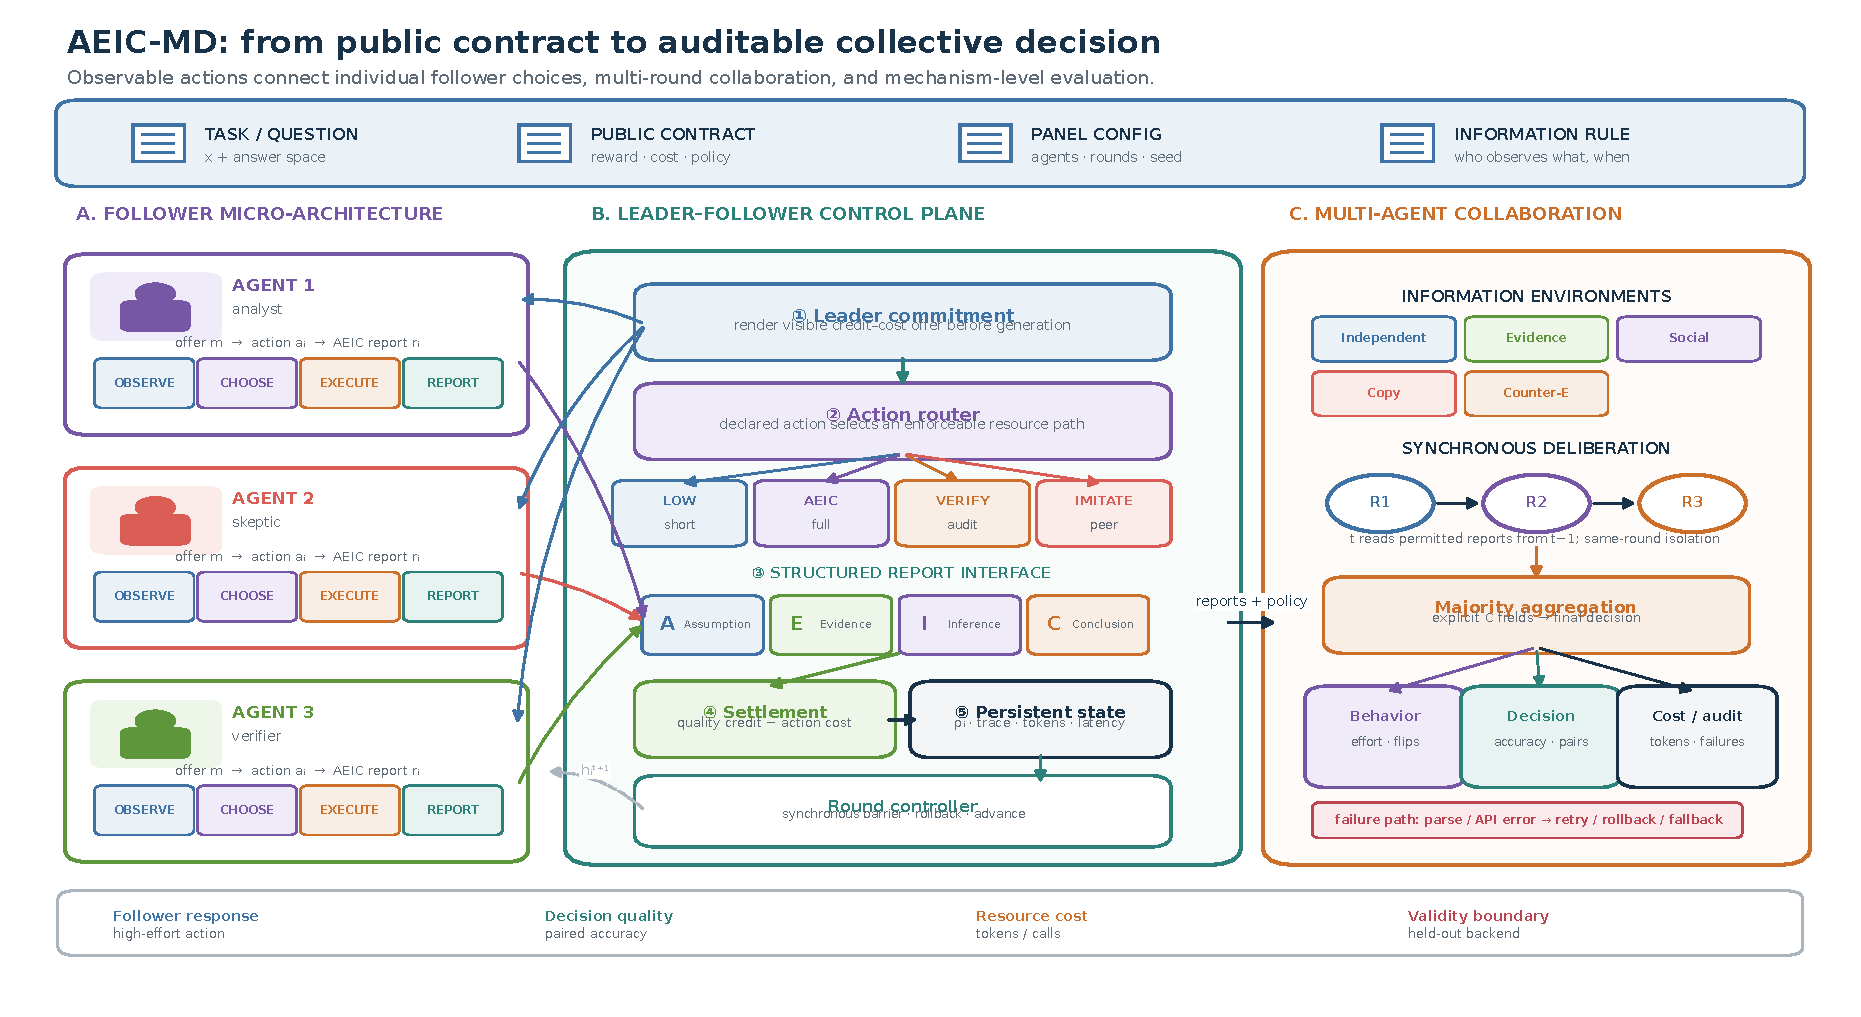
\includegraphics[width=\textwidth]{../figures/fig1_aeic_md_overview_rich.pdf}
\caption{AEIC-MD architecture. A public contract is rendered before followers choose resource-bearing actions. The selected path produces a structured AEIC report, after which the controller settles credit and cost, records state, and exposes only policy-permitted information to later rounds. The right-hand audit separates follower behavior, collective decision quality, and resource use.}
\label{fig:framework}
\end{figure}
